\chapter[Fundamentação Teórica]{Fundamentação Teórica}


\section{Modelo físico}

O problema abordado foi o do canal de Poiseuille. Ele pode ser definido como um escoamento em canal, com apenas uma dimensão finita no eixo $y$. Duas placas infinitas são definidas, perpendiculares ao eixo $y$. Nelas, o escoamento atinge velocidade igual a zero (condição de não deslizamento) e estão em regime de fluxo térmico constante. O eixo $z$ é definido como auto-similar tanto na velocidade quanto na temperatura, resultando em um domínio plano (Fig.\ref{figura.1}). O escoamento foi considerado incompressível e o fluido foi considerado newtoniano. O fluido escoa, em média, somente na direção do eixo $x$.
Os números de Reynolds ($Re = \frac{2R \overline{U}}{\nu}$) variam de $4560$ a $41441$, resultando em um regime turbulento.

\begin{figure}[h!]
	\centering
	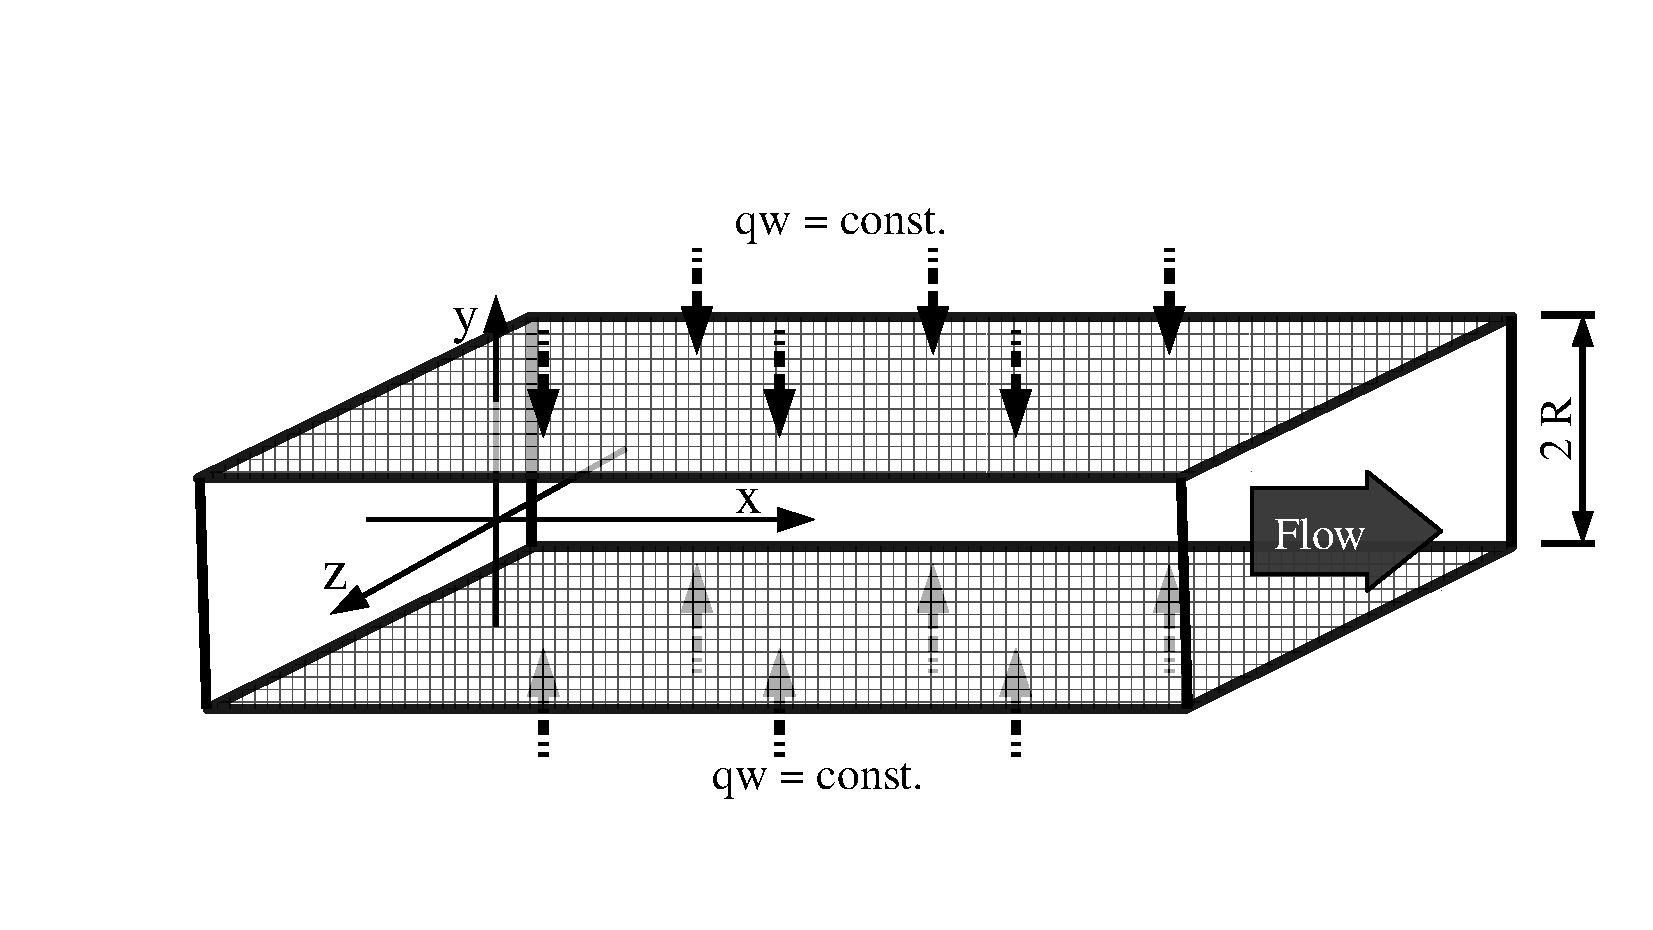
\includegraphics[angle=0, trim={0mm 23mm 0mm 35mm}, clip , scale=0.42]{cap_fundamentacao/canal1.pdf}
	\caption{Definição geométrica e condições de contorno.}
	\label{figura.1}
\end{figure}

Estas foram as suposições feitas para o problema proposto, que serão consideradas no modelo matemático diferencial adiante.

\section{Modelo matemático diferencial}
A formulação matemática do problema foi baseada nas equações de continuidade, de Navier-Stokes \cite{Cengel}, e na equação de transporte de energia térmica: 

\begin{equation}
  \frac{\partial u}{\partial t} + \frac{\partial u^2}{\partial x} + \frac{\partial uv}{\partial y} + \frac{\partial uw}{\partial z} = - \frac{1}{\rho} \frac{\partial {p}}{\partial x} + \nu \left( \frac{\partial^2 u}{\partial x^2} + \frac{\partial^2 u}{\partial y^2} + \frac{\partial^2 u}{\partial z^2}   \right)
\end{equation}

\begin{equation}
  \frac{\partial \rho}{\partial t} +  \frac{\partial (\rho u)}{\partial x} + \frac{\partial (\rho v)}{\partial y} + \frac{\partial (\rho w)}{\partial z} = 0
\end{equation}

\begin{equation}
  \frac{\partial T}{\partial t} + {\frac{\partial{}}{\partial{x}} (uT)} + {\frac{\partial{}}{\partial{y}} (vT)} + {\frac{\partial{}}{\partial{z}} (wT)}
  =
  {\frac{\partial{}}{\partial{x}}} \left(\alpha {\frac{\partial{T}}{\partial{x}}} \right) +
  {\frac{\partial{}}{\partial{y}}} \left(\alpha {\frac{\partial{T}}{\partial{y}}} \right) +
  {\frac{\partial{}}{\partial{z}}} \left(\alpha {\frac{\partial{T}}{\partial{z}}} \right)
\end{equation}

Sendo necessária esta definição para adimensionalização.
\begin{equation}\label{c_h_e}
  q_{conv.} = \dot{m} C_p \Delta T_m.
\end{equation}

\subsection{O estudo dos comportamentos médios}
Para simplificar o sistema, foi feito um tratamento estatístico nas equações. Cada grandeza foi dividida entre valor médio e flutuação da seguinte forma:


\begin{figure}[h!]
	\centering
	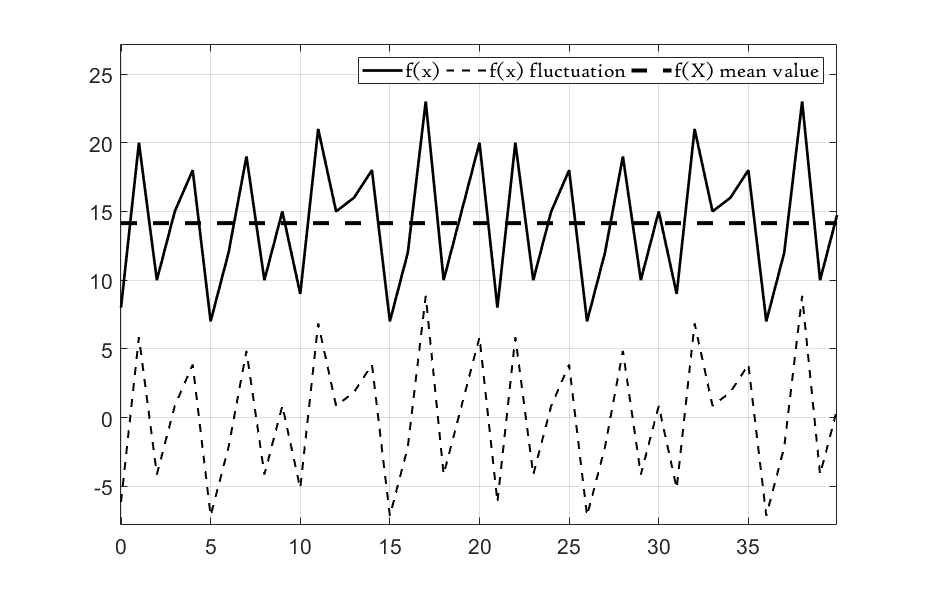
\includegraphics[angle=0, scale=0.60]{medios}
	\caption{Representação geométrica da separação entre os valores médios e as flutuações.}
	\label{figura.1}
\end{figure}

Dessa forma, aplicando as simplificações, obtêm-se as equações médias da continuidade (Eq.\ref{mass}), de Navier-Stokes (Eq.\ref{dynamics}) e de balanço de energia (Eq.\ref{energy permanent}) são apresentadas adiante:

\begin{equation}\label{mass}
\frac{\partial \overline{u}}{\partial x} = 0,
\end{equation}

\begin{equation}\label{dynamics}
\frac{\partial \overline{u} \, \overline{v}}{\partial y} = 
- \frac{1}{\rho} \frac{\partial \overline{p}}{\partial x} + \frac{\partial}{\partial y}\left(\nu \frac{\partial \overline{u}}{\partial y} - \overline{u^\prime v^\prime}\right),
\end{equation}


\begin{equation}\label{energy permanent}
\frac{\partial{}}{\partial{x}} \left(\overline{T^\prime u^\prime}\right) + \frac{\partial{}}{\partial{x}}\left(\overline{u} \overline{T}\right)     + 
\frac{\partial{}}{\partial{y}} \left(\overline{T^\prime v^\prime}\right) + \frac{\partial{}}{\partial{y}}\left(\overline{v} \overline{T}\right) 
=
{\frac{\partial{}}{\partial{x}}} \left(\alpha {\frac{\partial{\overline{T}}}{\partial{x}}} \right) +
{\frac{\partial{}}{\partial{y}}} \left(\alpha {\frac{\partial{\overline{T}}}{\partial{y}}} \right). 
\end{equation}

Sendo $\overline{u}$ e $\overline{v}$ as velocidades médias e $u^\prime$ e $v^\prime$ as flutuações na velocidade nos eixos $x$ e $y$, $\rho$ a massa específica, $\overline{p}$ a pressão média, $\nu$ a viscosidade cinemática, $\overline{T}$ a temperatura média, $T^\prime$ a flutuação na temperatura e $\alpha$ a difusividade térmica.

O método, independente da variável do tempo e baseado em comportamentos médios, é caracterizado como um exemplo de metodologia RANS (Reynolds-averaged Navier-Stokes).


\subsection{O regime permanente térmico}

O campo de velocidade média atinge um regime completamente desenvolvido e estatisticamente permanente no canal (Fig. \ref{figure.3}), mas o mesmo não ocorre para o campo de temperatura, pois um fluxo térmico constante é imposto sobre as paredes resultando no fato de que a temperatura continua aumentando no domínio, nunca se estabilizando.\\
Outra diferença entre os dois domínios é o fato de que o perfil de velocidade mantém-se constante no sentido do fluxo. Isso possibilita que o sistema seja representado unidimensionalmente, simplificando drasticamente as formulações matemáticas. O mesmo não pode ser dito para o campo de temperatura média, as temperaturas aumentam linearmente no sentido do fluxo (Fig. \ref{figure.2}):

\begin{figure}[h!]
	\centering
	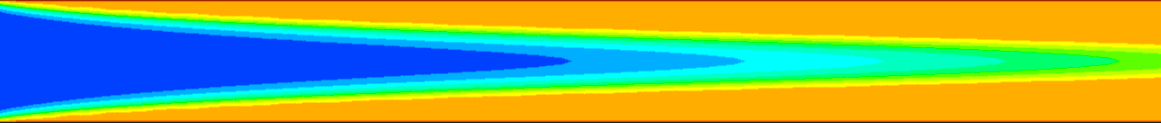
\includegraphics[angle=0, scale=0.4]{cap_fundamentacao/temperatura.png}
	\caption{Campo de temperatura média no canal de Poiseuille. O perfil de temperatura no canal aumenta linearmente na direção do fluxo.}
	\label{figure.2}
\end{figure}
\begin{figure}[h!]
	\centering
	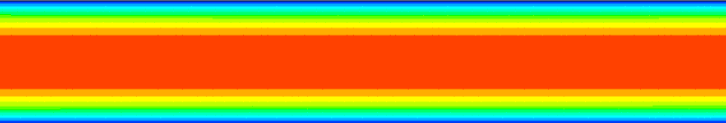
\includegraphics[angle=0, height=1.35cm , width=12.3cm]{cap_fundamentacao/velocidade.png}
	\caption{Campo de velocidade média no canal de Poiseuille. O perfil se mantém constante na direção do fluxo.}
	\label{figure.3}
\end{figure}


In a effort to simplify the solution, the thermal configuration was studied with a thermal energy balance (Eq. \ref{c_h_e}).

\begin{equation}\label{c_h_e}
q_{conv.} = \dot{m} C_p \Delta T_m,
\end{equation}

Where $q_{conv.}$ is the heat from convection, $\dot{m}$ the mass flux, $C_p$ the specific heat capacity and $T_m$ is the average temperature in a cross-section. 

\begin{equation}
2q_w b \Delta x = \dot{m} C_p \Delta T_m,
\end{equation}\\

